% This is a sample LaTeX input file.  (Version of 12 August 2004.)
%
% A '%' character causes TeX to ignore all remaining text on the line,
% and is used for comments like this one.

\documentclass{article}      % Specifies the document class

                             % The preamble begins here.
\title{\bf Principles of Computer Systems Design\\ {\Large Assignment 2}}  % Declares the document's title.
\author{Tudor Dragan\\
Gabriel Carp\\
Sokratis Siozos - Drosos}      % Declares the author's name.
\date{December 9, 2014}      % Deleting this command produces today's date.

\usepackage{verbatimbox}
\usepackage{listings}
\usepackage{color}
\usepackage[]{amsmath}
\usepackage[english]{babel}
\usepackage[utf8]{inputenc}
\usepackage{graphicx}
\usepackage{moreverb}
\usepackage{hyperref}
\usepackage[T1]{fontenc} % font
\usepackage{program}
\usepackage[top=1.5in, bottom=1.5in, left=1.4in, right=1.4in]{geometry}
\usepackage[super]{nth}

\definecolor{dkgreen}{rgb}{0,0.6,0}
\definecolor{gray}{rgb}{0.5,0.5,0.5}
\definecolor{mauve}{rgb}{0.58,0,0.82}

\lstset{frame=tb,
      language=Java,
      aboveskip=3mm,
      belowskip=3mm,
      showstringspaces=false,
      columns=flexible,
      basicstyle={\small\ttfamily},
      numbers=none,
      numberstyle=\tiny\color{gray},
      keywordstyle=\color{blue},
      commentstyle=\color{dkgreen},
      stringstyle=\color{mauve},
      breakatwhitespace=true
      tabsize=3
}
\newcommand{\ip}[2]{(#1, #2)}
                             % Defines \ip{arg1}{arg2} to mean
                             % (arg1, arg2).

%\newcommand{\ip}[2]{\langle #1 | #2\rangle}
                             % This is an alternative definition of
                             % \ip that is commented out.

\begin{document}             % End of preamble and beginning of text.

\maketitle                   % Produces the title.

\section*{Question 1: Recovery Concepts} 


\subsubsection*{1.In a system implementing force and no-steal, is it necessary to implement a scheme for redo? What about a scheme for undo? Explain why.}

In a system like this, we do not have to implement a scheme for redo because the force approach is used, which according to the theory means that we do not have to redo the changes of a committed transaction if there is a subsequent crash. As a result, all these changes are guaranteed to have been written to disk at the time the data has been committed. \\

If a no-steal approach is used, we also do not have to undo the changes of an aborted transaction (because these changes have not been written to disk). The no-steal approach assumes that all pages modified by ongoing transactions can be accommodated in the buffer pool, and in the presence of large transactions (typically run in batch mode, e.g., payroll processing), this assumption is unrealistic. \\

To implement a scheme for undo we need to have steal approach. Thus, if a frame is dirty and chosen for replacement, the page it contains is written to disk even if the modifying transaction is still active. 

\subsubsection*{2.  What is the difference between nonvolatile and stable storage? What types of failures are survived by each type of storage?}

A stable storage is guaranteed to survive crashes and media failures. Stable storage is implemented by maintaining multiple copies of information (perhaps in different locations) on nonvolatile storage devices such as disks or tapes. A non-volatile storage retains its content even if the power supply is interrupted, but has no guarantees because it can be prone to media failures. When power is again available, READ operations return the same values as before. A stable storage survives crashes and media failures, while the nonvolatile storage only survives crashes.\\


\subsubsection*{3.  In a system that implements Write-Ahead Logging, which are the two situations in which the log tail must be forced to stable storage? Explain why log forces are necessary in these situations and argue why they are sufficient for durability.}
The first situation for the log tail to be forced to stable storage is before a data page gets to disk. Another situation is when a transaction is committed, even if a no-force approach is being used. \\

A force approach is necessary because all the pages modified by the transaction, rather than a portion of the log that includes all its records, must be forced to disk when the transaction commits. Furthermore the cost of forcing the log tail is much smaller than the cost of writing all changed stages to disk, thus insuring durability.\\

\section*{Question 2: ARIES}

\begin{table}[h]
\begin{center}
\begin{tabular}{|c|c|c|c|c|}
\hline
\textbf{LSN} & \textbf{LAST\_LSN} & \textbf{TRAN\_ID} & \textbf{TYPE} & \textbf{PAGE\_ID} \\ \hline
1            & -                  & -                 & begin CKPT    & -                 \\ 
2            & -                  & -                 & end CKPT      & -                 \\ 
3            & NULL               & T1                & update        & P2                \\ 
4            & 3                  & T1                & update        & P1                \\ 
5            & NULL               & T2                & update        & P5                \\
6            & NULL               & T3                & update        & P3                \\
7            & 6                  & T3                & commit        & -                 \\ 
8            & 5                  & T2                & update        & P5                \\
9            & 8                  & T2                & update        & P3                \\ 
10           & 6                  & T3                & end           &                   \\ \hline
\end{tabular}
\caption{The LOG before the crash}
\label{The LOG before the crash}
\end{center}
\end{table}

\begin{enumerate}
\item %question 1 

To create the \emph{Transaction} and \emph{Dirty Page} tables we need to go through the \emph{Analysis Phase}. The algorithm states that we must reconstruct these tables after the last \emph{end CKPT} mark. We scan the log forward from \emph{LSN 3} and add the transactions in the \emph{Transaction Table} that have not encountered an \emph{end} record. We update the transaction's  \emph{last LSN} entry by updating it to the current LSN of the transaction. The \emph{Transaction table} after the analysis phase would look like this: \\

%transaction table
\begin{table}[h]
\begin{center}
\begin{tabular}{|c|c|c|}
\hline
\textbf{Tx ID} & \textbf{Status} & \textbf{LastLSN} \\ \hline
T1             & active          & 4                \\ 
T2             & active          & 9                \\ \hline
\end{tabular}
\caption{Transaction Table}
\label{Transaction Table}
\end{center}
\end{table}

For the \emph{Dirty Page table}, we need to check the \emph{update} records in the log. We need to store the earliest LSN for that page modification. If the a page is modified by a transaction that has successfully ended it's commit action, we remove it from the \emph{Dirty Page table}. The \emph{Dirty Page table} is presented below:\\

%dirty page table
\begin{table}[h]
\begin{center}
\begin{tabular}{|c|c|}
\hline
\textbf{Page ID} & \textbf{recLSN} \\ 
\hline
P2               & 3               \\
P1               & 4               \\
P5               & 5               \\ 
\hline
\end{tabular}
\caption{Dirty Page Table}
\label{Dirty Page Table}
\end{center}
\end{table}

\item %question 2
The transactions that have not committed, are considered \emph{losing transactions} because they have not been written to the non-volatile storage. In our case, the only transaction that completed it's commit is $T3$. Therefore, the loser transactions are $T1$ and $T2$.\\

\item %question 3
The REDO phase starts from the smallest \emph{recLSN} in dirty page table after the Analysis phase. In our case the smallest LSN is \emph{3}. The UNDO phase ends at the oldest log record of an active transaction at crash. In our case the minimum LSN is \emph{3}.\\

\item %question 4
Because in the REDO phase we actually reapply everything, all the pages that were updated after the checkpoint will be modified. The set should therefore be:
\begin{verbatim}
RedoPageSet = {P2,P1,P5,P3}
\end{verbatim}

\item %question 5
In the UNDO stage we need to rollback all the transactions that haven't committed their changes. The UNDO set is composed of the LSN's that are attributed to a loser transaction. In our case the UNDO log record set will be:
\begin{verbatim}
UndoLogRecords = {9,8,5,4,3}
\end{verbatim}

\item %question 6
When building the log after a crash we must rollback the transactions that haven't committed (loser transactions). Thus, we must add CLR records to the log to undo the modifications that a loser transaction has made. the log table after the recovery procedure will look like this:

\begin{table}[h]
\begin{center}
\begin{tabular}{|c|c|}
\hline
\textbf{LSN} & \textbf{LOG}         \\ \hline
1            & begin CKPT           \\ \hline
2            & end CKPT             \\ \hline
3            & update: T1 writes P2 \\ \hline
4            & update: T1 writes P1 \\ \hline
5            & update: T2 writes P5 \\ \hline
6            & update: T3 writes P3 \\ \hline
7            & T3 commit            \\ \hline
8            & update: T2 writes P5 \\ \hline
9            & update: T2 writes P3 \\ \hline
10           & T3 end               \\ \hline
\textbf{X}   & \textbf{CRASH}       \\ \hline
11           & CLR: Undo T2 LSN 9   \\ \hline
12           & CLR: Undo T2 LSN 8   \\ \hline
13           & CLR: Undo T2 LSN 5   \\ \hline
14           & T2 End               \\ \hline
15           & CLR: Undo T1 LSN 4   \\ \hline
16           & CLR: Undo T1 LSN 3   \\ \hline
17           & T1 End               \\ \hline
\end{tabular}
\caption{Log after Recovery}
\label{Log after Recovery}
\end{center}
\end{table}
\end{enumerate}
To add the CLR records we must keep track of the last LSN's of the loser transactions. We choose the largest LSN ( in out case 9) and we observe that the record is an \emph{update}. We then undo the update and write a CLR (Compensation Log Record) to record that we did the rollback. Afterwards we update the CLR's prevLSN with the last LSN of the transaction (in our example here, we set the prevLSN to 8). We apply this algorithm until we have no more loser transaction updates to undo. \\

\section*{Programming Task}

\subsection*{Questions for Discussion on the Performance Measurements}

We initialize the bookstore with 50 books. The number of books that clients can buy is set to 5, while the number of book copies is set to 1. After some tests it was clear that since the probability of buying a book was higher than the one for adding books or book copies then as the number of concurrent clients increased, the "goodput" was steadily decreasing. As a result, we set the variable numAddCopies to 8 (a value eight times higher than the numBookCopiesToBuy) so that we can make sure that the sale misses are minimized.  The variable numBooksToAdd was set to 5, which is the same with numBooksToBuy, test whether the sale misses increased or not. Finally, the variable numBooksWithLeastCopies was also set to 5 for the same reason as before.\\

We ran the tests in a Macbook Pro with 2Ghz Intel core i7(8 threads) and 8GB of RAM. The testing was done for 1 and up to 10 concurrent clients in both local and through RPC. \\

We tested the the bookstore for multiple values of numEditorPicksToGet, numAddCopies and numBooksToAdd. We did not change the number of warmUpRuns or numActualRuns so that we could have a better idea of the impact that these changes had on the final results.\\

Below each group of graphs we give the specific workload configurations that we used.\\

The tests were done locally and using proxies that connected to the CertainBookStore server. We defined each test by "goodput" and latency. The graphs on the left are the graphical representation of the "goodput" and throughput and the graphs on the right represent the latencies for each number of clients. Our tests simulate between 1 and 10 clients that interact with the store concurrently. We decided to separate the plots between the local and remote environment because the differences between the values were too high.\\

The latency plots came out as we expected. Both in the local and remote tests the latency increased steadily (with minor deviations) when the number of clients increased. This increase of clients added an overhead to the response time of each request.\\

The throughput has a different pattern. In the local tests we observed that the successful throughput peaked when the number of threads was in the 4-6 range. The throughput steadily declines after this mark until it reaches almost the same levels as using one client. However, the remote tests perform very differently.\\

\begin{figure}[ht]
\centering
 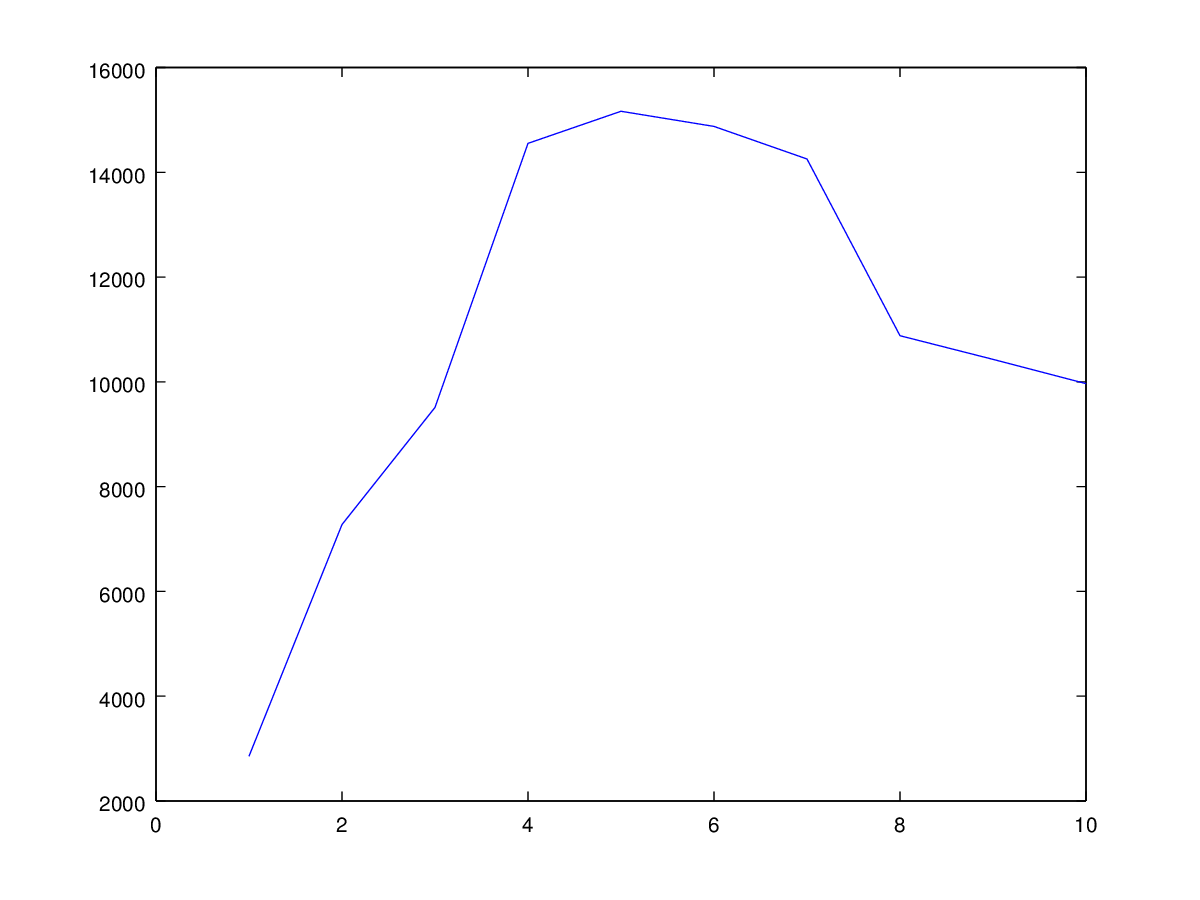
\includegraphics[scale=.33]{graphs/graph1-goodput}
 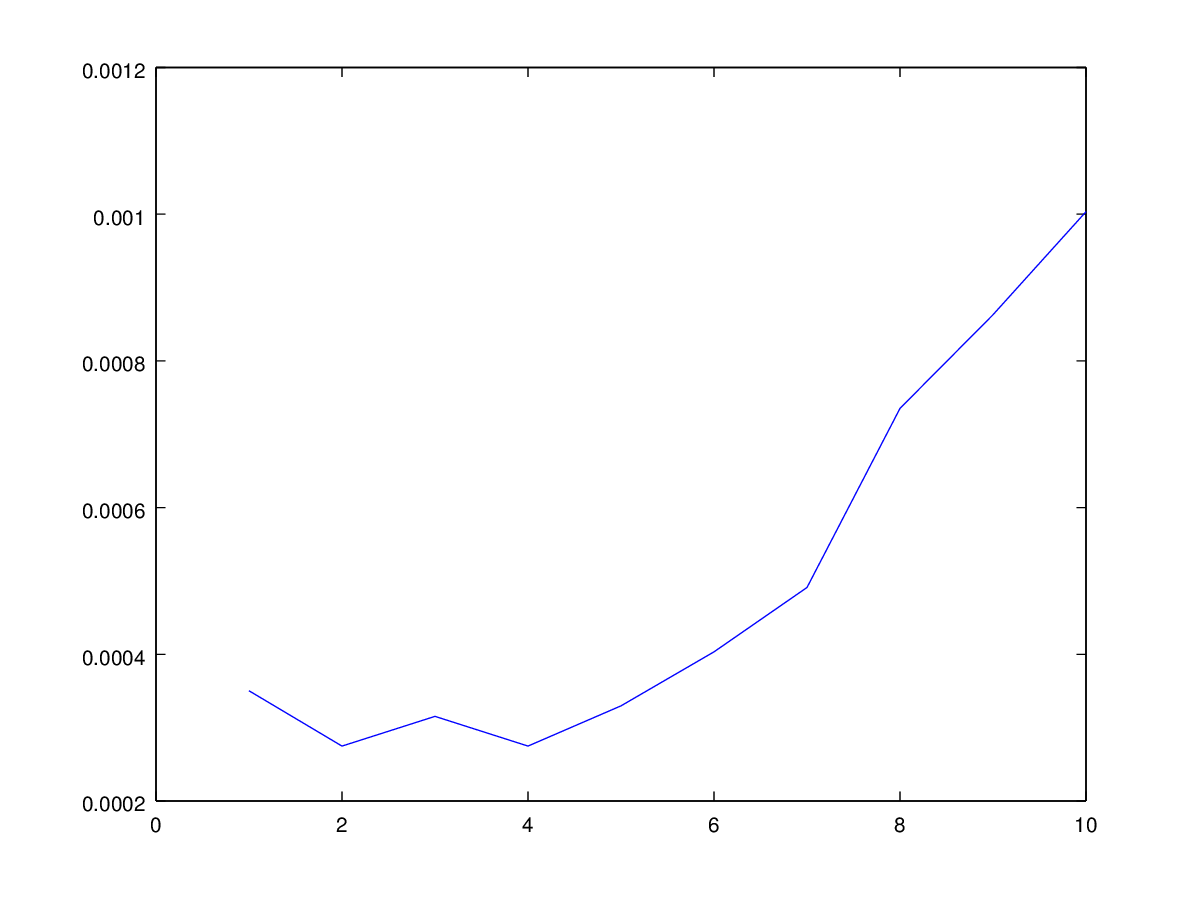
\includegraphics[scale=.33]{graphs/graph1-latency}
\caption{Test 1: Local goodput/throughput and latency \label{overflow}}
\end{figure}

\begin{figure}[ht]
\centering
 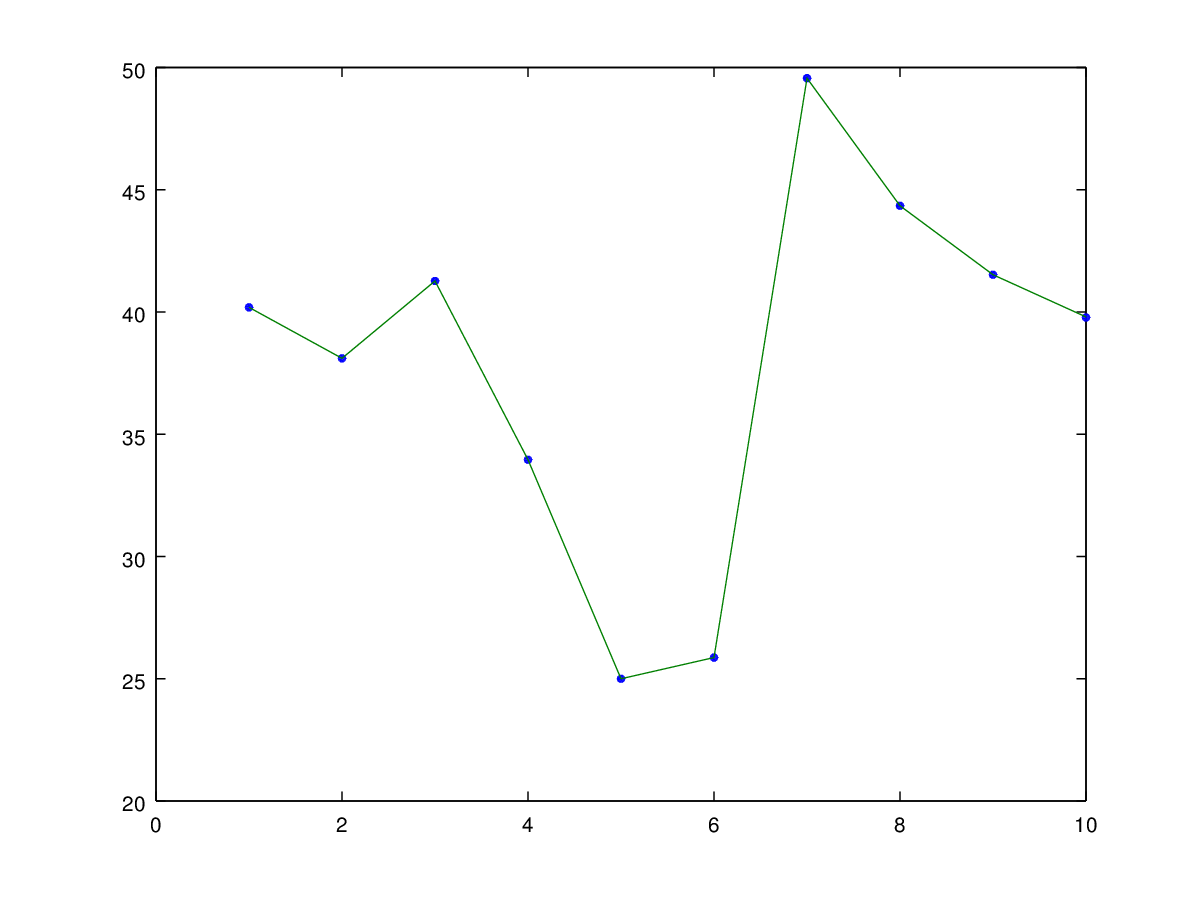
\includegraphics[scale=.33]{graphs/graph2-goodput}
 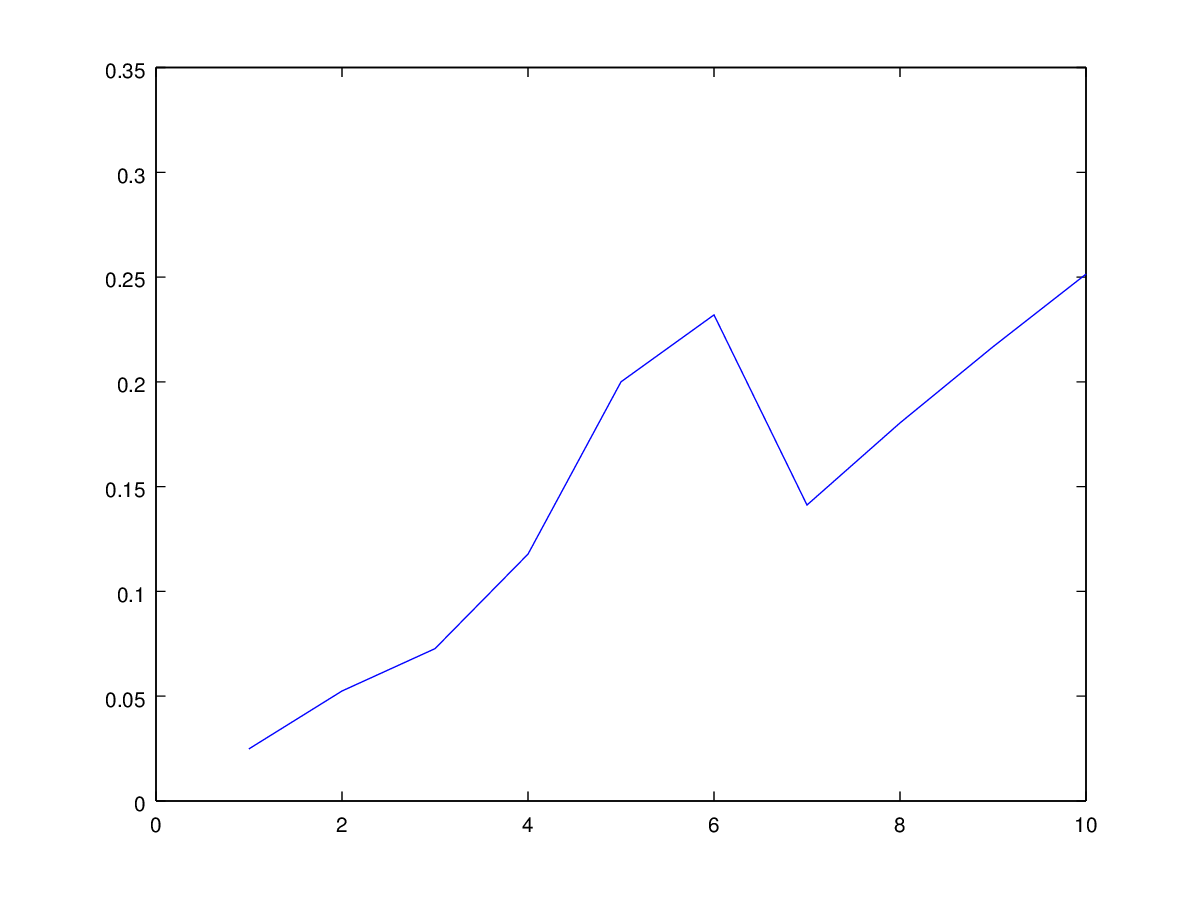
\includegraphics[scale=.33]{graphs/graph2-latency}
\caption{Test 1: Remote goodput/throughput and latency \label{overflow}}
\end{figure}

\begin{verbatim}
private int numBooksToBuy = 5;
private int numBookCopiesToBuy = 1;
private int numEditorPicksToGet = 10;
private int numAddCopies = 8;
private int numBooksToAdd = 5;
private int numBooksWithLeastCopies = 5;
private int warmUpRuns = 100;
private int numActualRuns = 500;
private float percentRareStockManagerInteraction = 10f;
private float percentFrequentStockManagerInteraction = 30f;
\end{verbatim}


\begin{figure}[ht]
\centering
 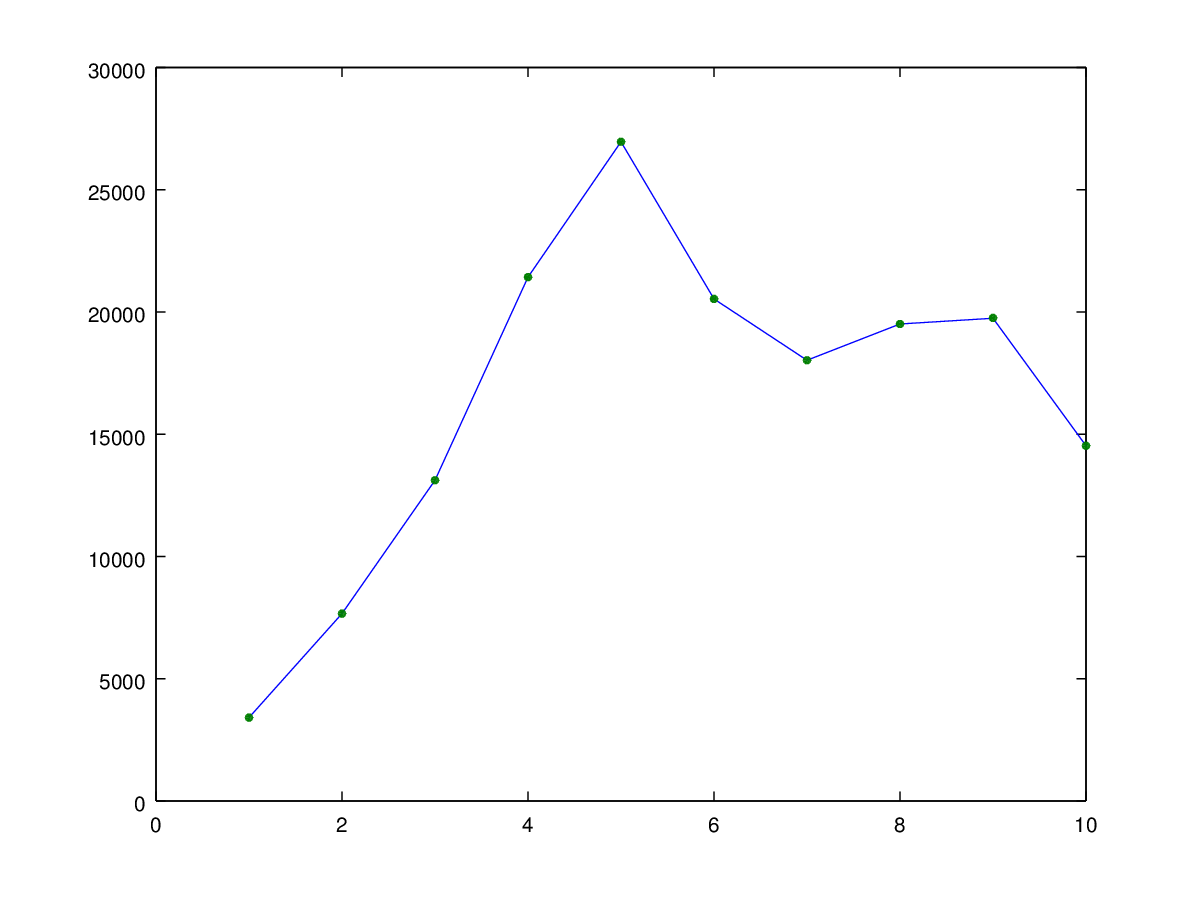
\includegraphics[scale=.33]{graphs/graph3-goodput}
 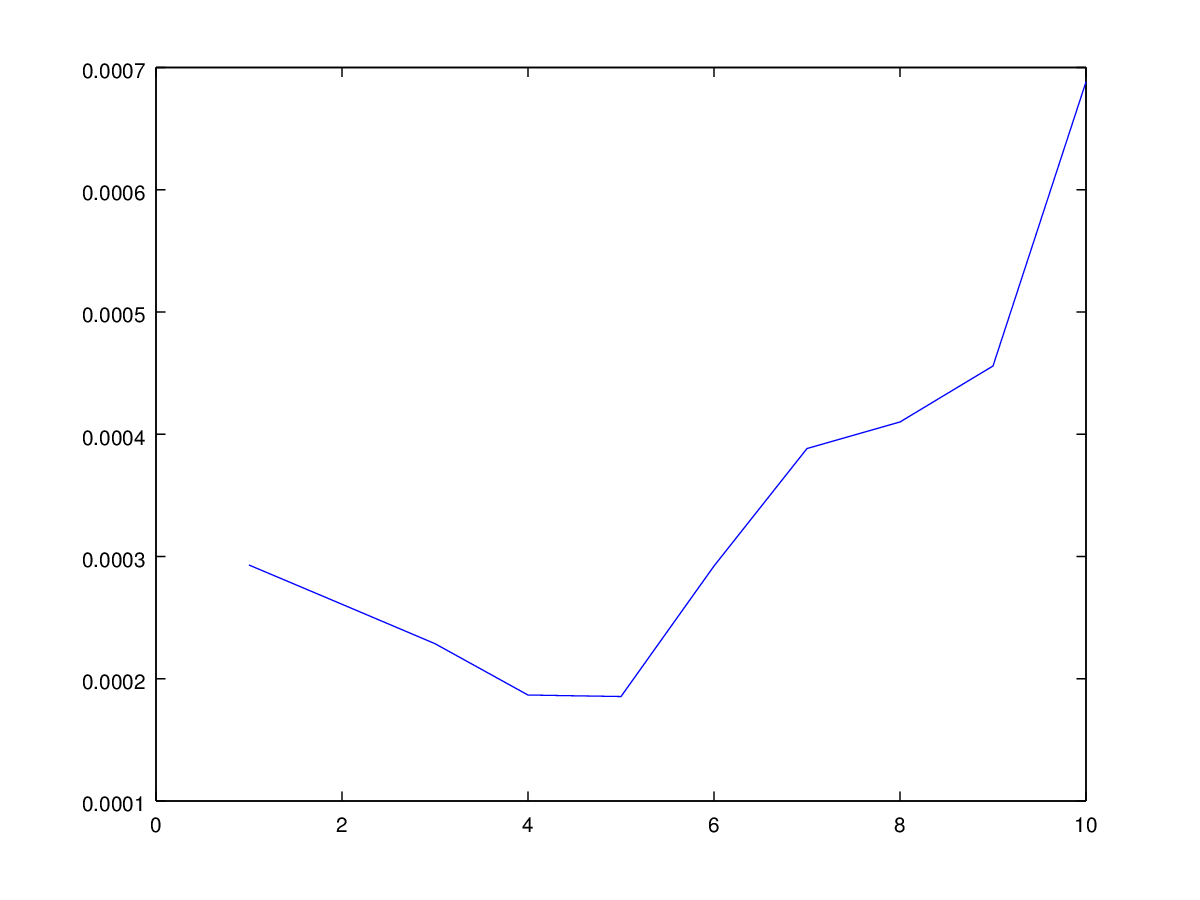
\includegraphics[scale=.33]{graphs/graph3-latency}
\caption{Test 2: Local goodput/throughput and latency \label{overflow}}
\end{figure}

\begin{figure}[ht]
\centering
 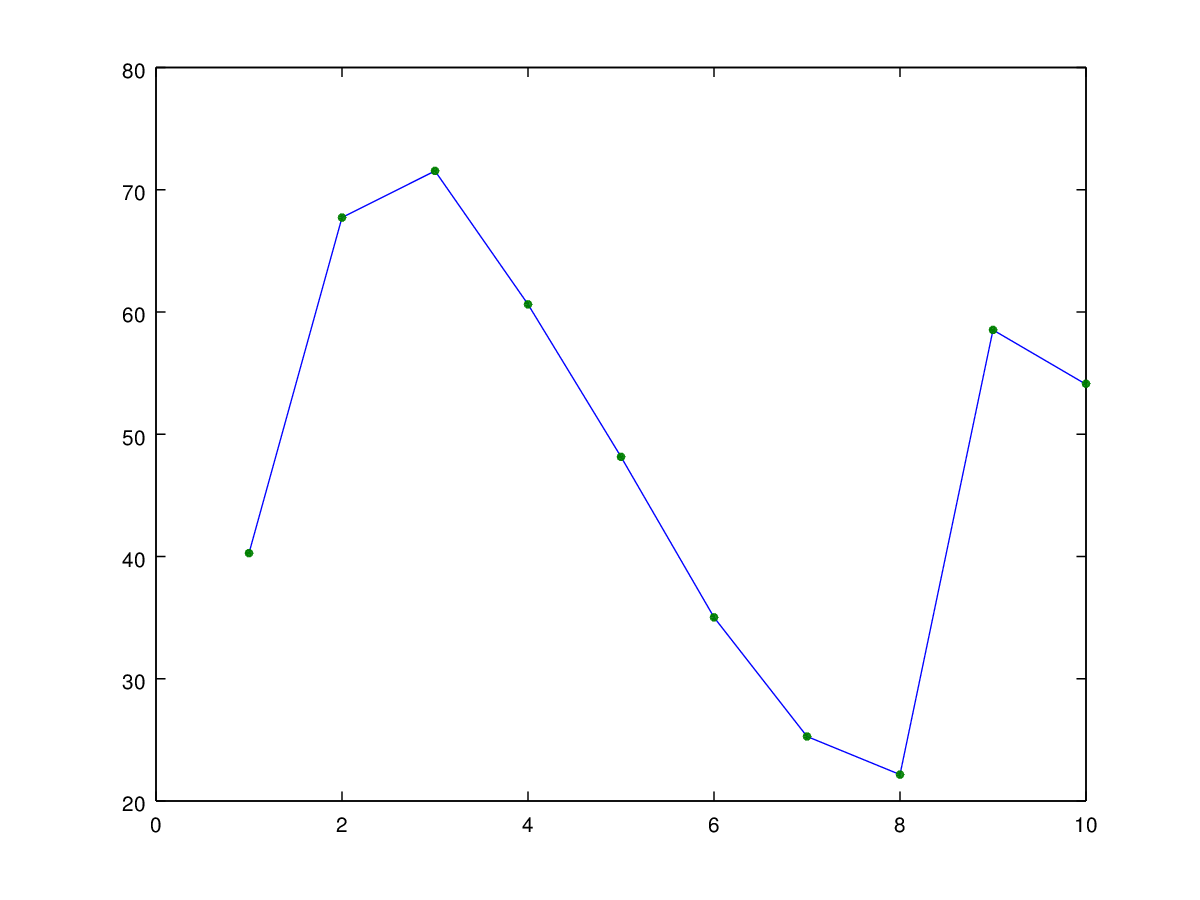
\includegraphics[scale=.33]{graphs/graph4-goodput}
 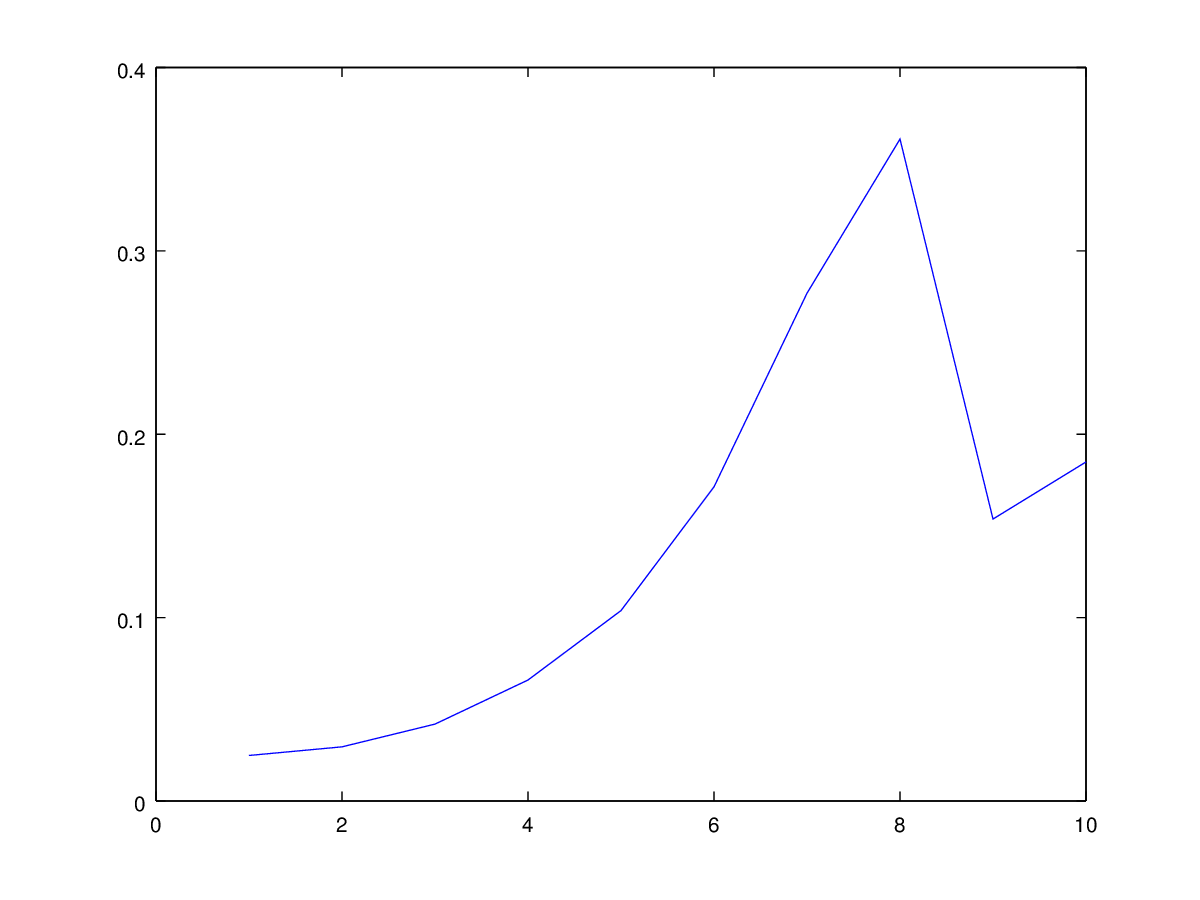
\includegraphics[scale=.33]{graphs/graph4-latency}
\caption{Test 2: Remote goodput/throughput and latency \label{overflow}}
\end{figure}

\begin{verbatim}
private int numBooksToBuy = 5;
private int numBookCopiesToBuy = 1;
private int numEditorPicksToGet = 5;
private int numAddCopies = 5;
private int numBooksToAdd = 3;
private int numBooksWithLeastCopies = 5;
private int warmUpRuns = 100;
private int numActualRuns = 500;
private float percentRareStockManagerInteraction = 10f;
private float percentFrequentStockManagerInteraction = 30f;
\end{verbatim}

\begin{figure}[ht]
\centering
 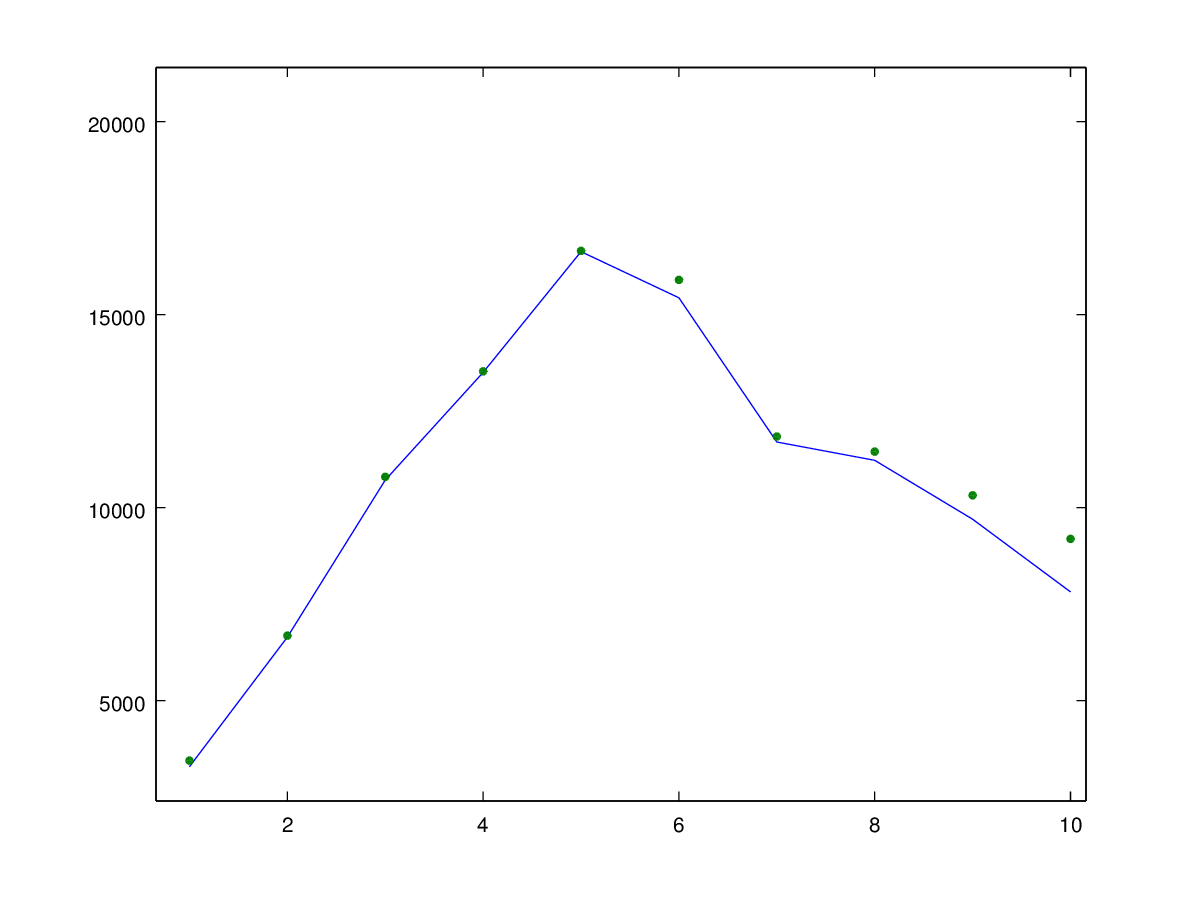
\includegraphics[scale=.33]{graphs/graph5-goodput}
 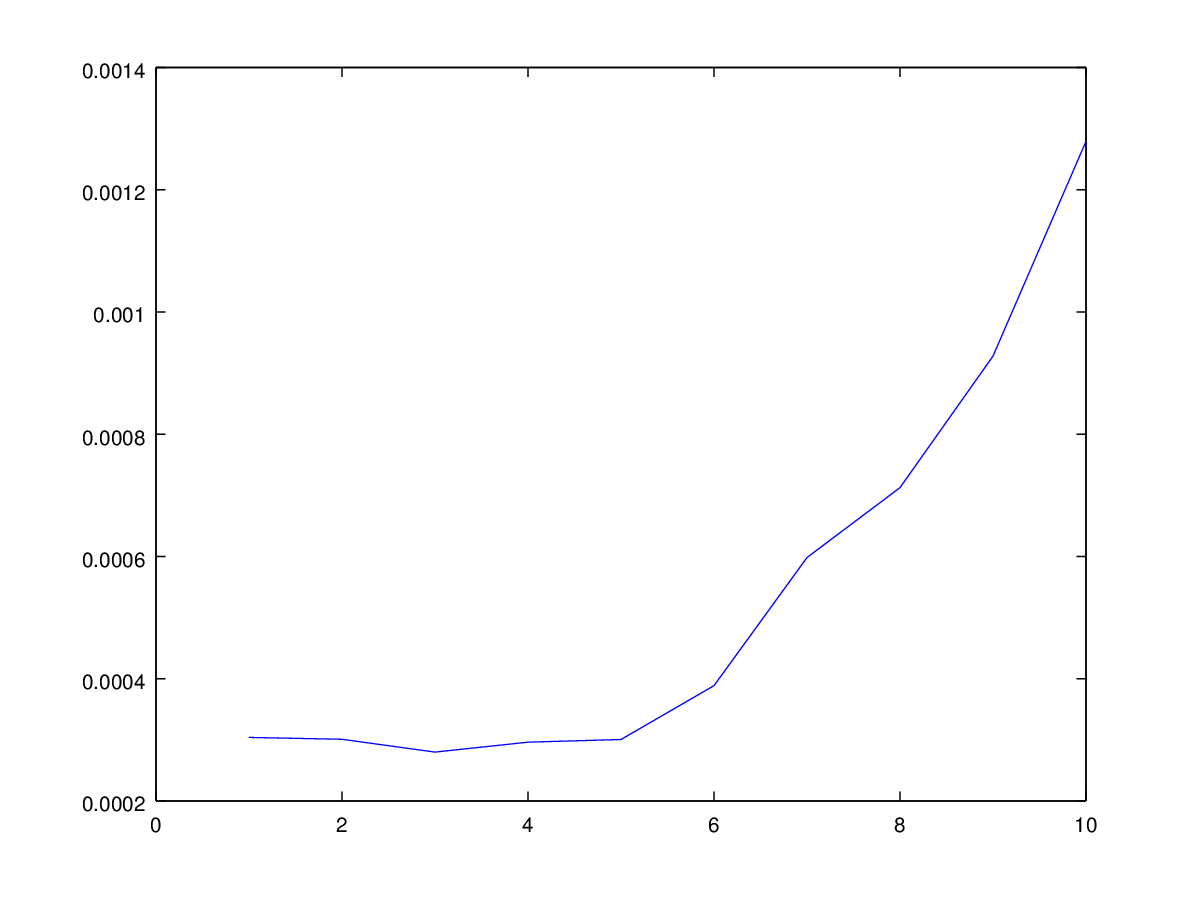
\includegraphics[scale=.33]{graphs/graph5-latency}
\caption{Test 3: Local goodput/throughput and latency \label{overflow}}
\end{figure}

\begin{figure}[ht]
\centering
 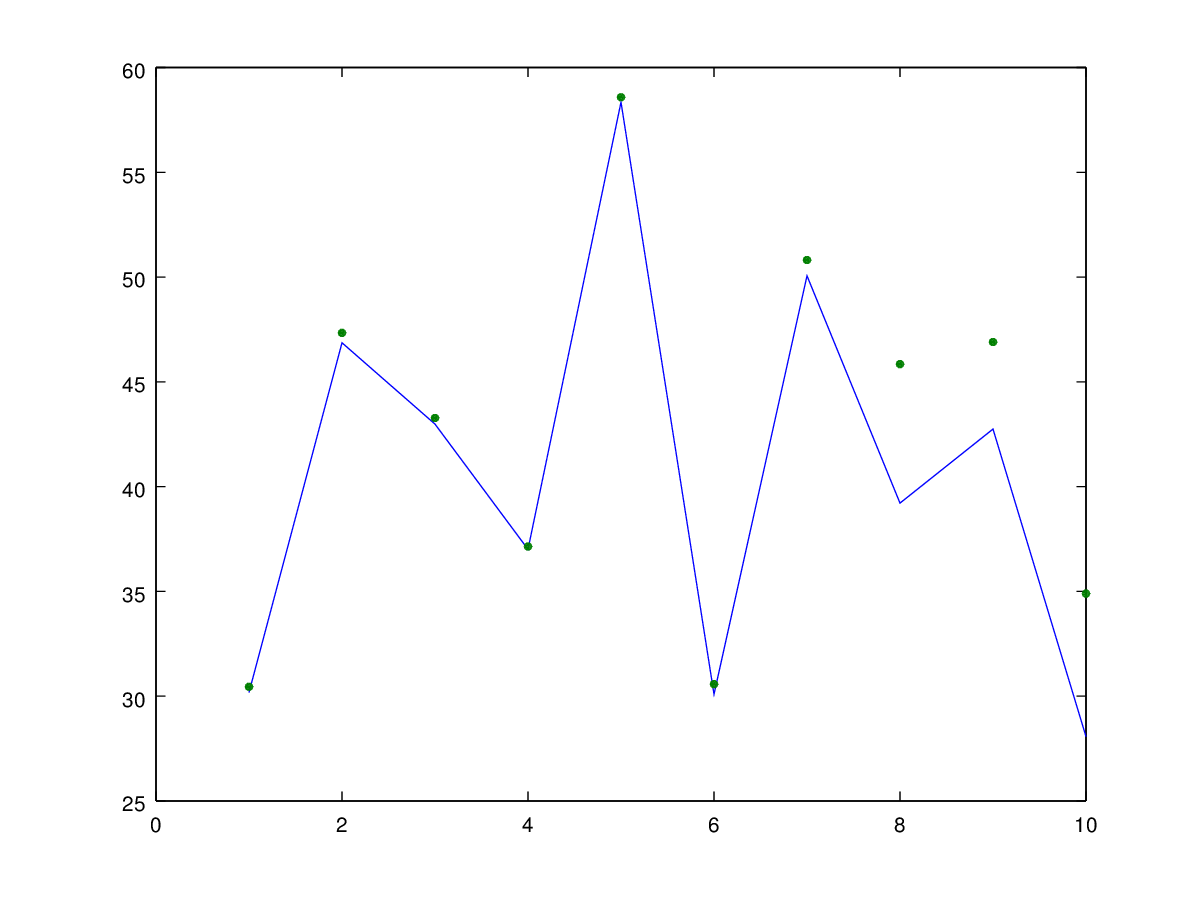
\includegraphics[scale=.33]{graphs/graph6-goodput}
 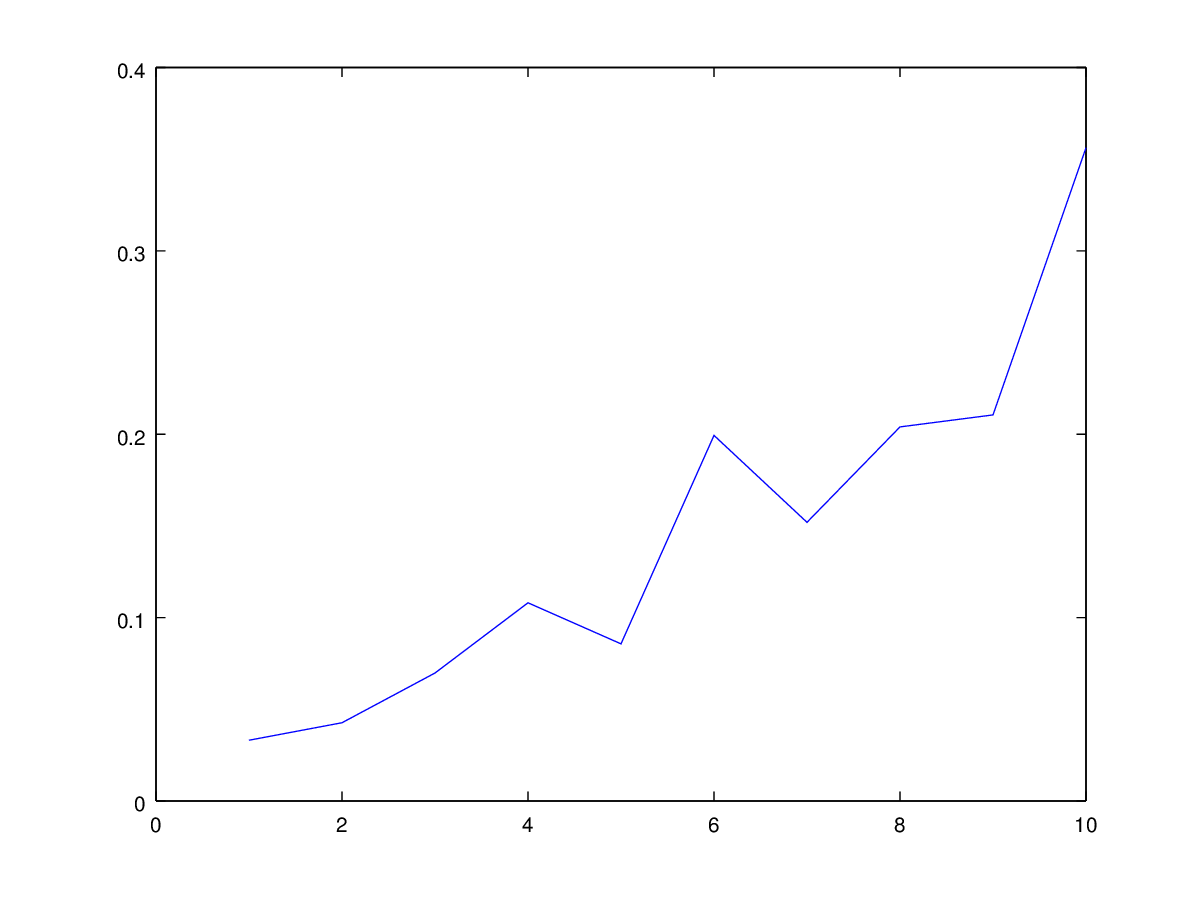
\includegraphics[scale=.33]{graphs/graph6-latency}
\caption{Test 3: Remote goodput/throughput and latency \label{overflow}}
\end{figure}

\begin{verbatim}
private int numBooksToBuy = 3;
private int numBookCopiesToBuy = 2;
private int numEditorPicksToGet = 5;
private int numAddCopies = 6;
private int numBooksToAdd = 5;
private int numBooksWithLeastCopies = 5;
private int warmUpRuns = 100;
private int numActualRuns = 500;
private float percentRareStockManagerInteraction = 10f;
private float percentFrequentStockManagerInteraction = 30f;
\end{verbatim}
 
According to the theory, a performance metric is considered reliable if a system A outperforms a system B when the corresponding values of the metric for both systems indicate that system A should outperform system B. \\

Based on the graphs we can safely infer that latency is a reliable metric as we can see that as we increase the number of concurrent clients, the latency does too. As for for the throughput we cannot say that it is a reliable metric. As we can see from the graphs there is no correlation between the number of clients and throughput, even after configuring the workload metrics. \\

An additional metric that could be used to demonstrate the performance of the book-store is the Execution time. Since it can give precise results concerning the time it took for the system to execute a given program or a unit test. This way, as the theory says, we can compare time directly, or use them to derive appropriate rates. \\

Another metric that could be used is the Speedup metric. Although, it is defined in terms of throughput, it is often calculated directly from execution times. As a result, we can safely say that it is a reliable metric for our system. \\

\end{document}               % End of document.